% MDS stuff

\label{chap-mds}

\section{Introduction}

Cary on from previous chapter, need data-dependent way of doing transform...

\subsection{Proposition}

Multidimensional scaling (MDS) or, as it is often referred to, principle coordinates (PCO) (\cite{gower1966}) is a method used in multivariate analysis. It is closely related to techniques such as PCA (\cite{chatfieldcollins}, p. 200) and canonical correspondence analysis (\cite{terbraak}). The starting point for MDS is a matrix of distances, representing some kind of dissimilarity between observations. This distance could be calculated from the data, for example ideological distance between politicians measured using NOMINATE scores (\cite{quantss}, p. 225), or could instead be distances that occur in the data naturally through experimental setup,  for example comparative distances between stimuli response in a psychophysical experiment (\cite{torgerson}). Here we concentrate on geographical distances.

MDS takes this matrix of distances and projects the data in such a way that Euclidean inter-point distances in the projection are approximately the same as the distances in the matrix (\cite{chatfieldcollins}, p. 187). If the matrix of distances is of rank $m$ then the projection can be in $m-1$ or less dimensions; a projection into 2 dimensions is a typical choice, since it is easily visualised. For this reason one can also think of MDS as a dimension reduction technique, finding a projection of a data cloud into lower dimensional space, while still retaining information about the disimilarities between the points.

When MDS is performed on some categorised set of dissimilarities (as is often the case in social science and psychology) it is referred to as non-metric MDS, where as on a continuous scale it is known as metric MDS. Though they have different names, the calculations are identical (aside from the method of finding the distances.) Discussion here will focus on metric MDS.

Multidimensional scaling offers a framework for finite area smoothing over a region with a complex boundary. Given the set of distances between points in a domain, we can project those points into a configuration such that the distances between those points are approximately preserved. Now, if the Euclidean metric were to be used to calculate the distances between the points then the result from the projection would be identical to the starting point configuration (provided that we projected back into the same number of dimensions). However, if it were possible to use a metric that took into account the distance within the boundary (a within-area distance) then the resulting configuration of points would (approximately) respect the boundary of the domain.

Justification for this approach is as follows. In many applications within-area distances is meaningful, given that there is some reasoning behind why certain parts of the domain should not affect one another. Biological populations respect the intrinsic structure of these domains and in general do not respect Euclidean geometry in their movement patterns. When within-area distances are meaningful, it makes sense to use information about the structure of the domain rather than discard it and use the somewhat arbitrary choice of Euclidean geometry. However, as literature on smoothing is firmly based in a Euclidean context, it would be preferable to perform the smoothing in Euclidean space. In this case the approximation to Euclidean space afforded by an MDS projection of the within-area distances offers a bridge between these two requirements.

\subsection{Procedure}
\label{mdsproc}
Given a sample $\{\mathbf{x}_i, z_i : i=1\dots n\}$, the set of points in the domain over which smoothing is to be performed, $\mathbf{x}_i$ is the location (a $k$-vector, although here 2-vectors are assumed throughout) of the $i^\text{th}$ point with response $z_i$ (assumed to be univariate). Here, finding an MDS configuration of a set of points consists of: $i$) calculating the within-area distances between the points, $ii$) forming the distance matrix and, $iii$) actually performing the MDS projection.

\begin{enumerate}
\item Obtain the MDS configuration for the domain using some representative set of points over the area in question. The only use of the MDS locations obtained in this step is to define the configuration, they are discarded afterward. Representative points could be a sparse grid over the domain or subset of $\{\mathbf{x}_i : i=1\dots n\}$; more detail and justification is provided in section \ref{grids}, below.

\item Using the MDS configuration obtained above along with Gower's interpolation (see section \ref{gowers}) obtain the location of the sample in the MDS configuration: $\{\mathbf{\tilde{x}}_i, z_i : i=1\dots n\}$.

\item Smooth $\{\mathbf{\tilde{x}}_i, z_i : i=1\dots n\}$ using a regression spline.

\item To predict at a location $\mathbf{x_j}$ in the original domain, use Gower's interpolation to 
obtain the point's location in the MDS space: $\mathbf{\tilde{x}}_j$. Predict $\hat{z}_j$ at $\mathbf{x}_j$ using the smooth at $\mathbf{\tilde{x}}_j$.
\end{enumerate}

The rest of this chapter is structured as follows: in \secref{MDStechdet} an overview of MDS is given, along with technical details of how the MDS configuration is calculated; \secref{mdsdist} focuses on how the within-area distances are found; \secref{mdssims} shows some examples of this method on simulated data. Finally \secref{MDSimprov} shows some improvements to the initial method and further simulations.


\section{Technical details}
\label{MDStechdet}

The basic concept behind MDS is to take the data, calculate their within-area inter-point distances and then find their points in a new coordinate system based on those inter-point distances. Their new positions are determined by finding the eigen-decomposition of the (centred) matrix of distances between points. First a description of the MDS procedure when Euclidean distances are used is given, followed by the justification for the use of the same procedure when using within-area distances. 

\subsection{Finding the new point configuration}

First define $d_{ij}$ as the distance between the points $i$ and $j$. These are used to form a (symmetric) matrix, $D$, with \ijth element $d^2_{ij}$. For the moment let us assume that $D$ is known and $d_{ij}$ is the Euclidean distance between points $i$ and $j$. 

\cite{diaconis08} gives a clear definition of the algorithm (due to \cite{schoenberg35} and \cite{torgerson}) for finding the new locations of points, which is outlined below. Further detail is given in \cite{principlesofMA}, pp. 104-108 and \cite{chatfieldcollins}, pp. 189-200.

First, suppose that the $n$ unknown new locations (in $n$ dimensions) in our MDS configuration are entries in an $n \times n$ matrix, $\tilde{X}^*$. Now let $S=\tilde{X}^{*} \tilde{X}^{*\text{T}} $, so $S$ is a matrix of scalar products of the point vectors, \emph{ie.} the \ijth element of $S$ is:
\begin{equation}
s_{ij} = \mathbf{x}_i\tr{\mathbf{x}_j},
\label{selem}
\end{equation}
$S$ is an $(n\cross n)$ matrix. Note that we may only find $\tilde{X}^*$ up to a translation and rotation, so it is assumed that the values in $\tilde{X}^*$ have been centred about the origin.

We now wish to relate $D$ to $S$. First, note that that \ijth element of D is 
\begin{equation}
d_{ij}^2 = (\mathbf{x}_i-\mathbf{x}_j)\tr{(\mathbf{x}_i-\mathbf{x}_j)} = \mathbf{x}_i\tr{\mathbf{x}_i} + \mathbf{x}_j\tr{\mathbf{x}_j}  -2 \mathbf{x}_i\tr{\mathbf{x}_j}.
\label{dij}
\end{equation}
Using \eqn{selem}, we can re-write \eqn{dij} as
\begin{equation}
D=\mathbf{s}_\text{diag}\tr{\mathbf{1}} + \mathbf{1}\tr{\mathbf{s}_\text{diag}} -2S.
\label{dijmat}
\end{equation}
where $\mathbf{1}$ is an $n \cross 1$ vector of 1s and $\mathbf{s}_\text{diag}$ is the $n \cross 1$ vector of diagonal elements of $S$.

Defining:
\begin{equation}
H = I-\frac{1}{n}\mathbf{1}\tr{\mathbf{1}},
\end{equation}
where $I$ is the identity matrix, as usual, and $\mathbf{1}\tr{\mathbf{1}}$ is an $n \cross n$ matrix of 1s.

By pre- and post-multiplying any matrix by $H$ the matrix is double centred (such that row and column means are 0). Pre- and post-multiplying \eqn{dijmat} by $H$ yields:
\begin{equation}
HDH = -2HSH.
\end{equation}
The first two terms in on the right hand side of \eqn{dijmat} are zero since the rows of $\mathbf{s}_\text{diag}\tr{\mathbf{1}}$ and the columns of  $\mathbf{1}\tr{\mathbf{s}_\text{diag}}$ are constant. Since $S$ is already centred so $HSH=S$. Rearranging, the following relation between $S$ and $D$ holds:
\begin{equation}
S = -\frac{1}{2}HDH.
\end{equation}

Now there is a relation between $D$ and $S$, we ca concentrate on dealing with $S$. In order to find $\tilde{X}^{*}$ we must factor $S$. There are many options for matrix decomposition. One option for factoring $S$ is to use the Cholesky decomposition, however, with MDS we are looking to decompose the space based on the directions of largest variation, \emph{ie.} those that have the largest contribution to $s_{ij}$. For that reason we use the eigen-decomposition.

Finding the eigen-decomposition of $S$, we obtain $S=U\Lambda\tr{U}$. Here $U$ is the $n \cross n$ orthogonal matrix of eigenvectors and $\Lambda$ is the $n \cross n$ diagonal matrix of eigenvalues. Then $\tilde{X}^*$ maybe computed as:
\begin{equation}
\tilde{X}^*=U\Lambda^{\frac{1}{2}}.
\end{equation}

Following these steps $\tilde{X}^*$ is an $n \cross n$ matrix. Multidimensional scaling is performed to reduce the dimensionality of the data and, indeed, the aim here is to smooth in two dimensions. To represent the space using two dimensions the directions with the two largest eigenvalues are chosen and the others discarded. These two largest eigenvalues and their associated eigenvectors constitute the two largest sources of variation in distance (since they are the two largest contributions to $S$) this gives the two dimensional representation of the data. 

Defining $\tilde{X}$ to be the $n \cross 2$ dimensional matrix obtained from truncating the full new coordinate set to the first two columns in decreasing eigenvalue order, a 2-dimensional representation has been obtained. More generally, we can reduce the $\tilde{X}^*$ to an $n \cross k$ matrix, where $k$ is the chosen dimensionality of the MDS space.

In summary, to calculate the MDS configuration of a set of points (given their inter-point distances) we merely need to double centre the matrix of distances and perform an eigen-decomposition on the resulting matrix, $S$. 

For finite area smoothing, $d_{ij}$ should be the shortest distance between the points, given the path between any pair of points remains within the domain. Calculation of the inter-point distances is covered in \secref{mdsdist}, however it is important to first justify the use of these steps when non-Euclidean distances are used. 

One can think of the justification in the following way: given that the distances in $D$ obey the triangle inequality, all of the points in $D$ ($n$ of them if $D$ is $n \cross n$) may be represented in $n$ dimensional Euclidean space (at worst.) Hence, in the case where the $d_{ij}$ are Euclidean distances in two dimensions, the smallest dimensional space in which they can be represented is 2, but they may still reside in $n$-dimensional space with no loss of information about the distances. So, in the case when the distances in $D$ are shortest within-area distances, one can think of the points in $D$ as residing in a higher number of dimensions in such a way that the distances between them are Euclidean.

Note that an additive constant can be computed and added to the non-diagonal entries of $D$ to ensure that the eigenvalues of $S$ are non-negative. However, this does not occur in any of the examples shown here.

\subsection{Gower's interpolation} 
\label{gowers}
Given the setup in \secref{mdsproc}, once the MDS configuration has been found, further points will need to be inserted into our MDS representation. For example when further data is collected, or in order to predict over points not in the initial grid. In this case we would like to insert those new points into the configuration given by MDS. A number of methods have been developed over the past 40 years; Gower's interpolation (\cite{gower1968}) is covered here.

Say we have some point, $x_{\text{new}}$ and we wish to find its new location, $\tilde{x}_{\text{new}}$ in the MDS configuration, $\tilde{X}$. The position of $\tilde{x}_{\text{new}}$ is at a distance from the points in $\tilde{X}$ which is approximately the same as that of $x_{\text{new}}$ to the points in the non-transformed space. 

Note that here we are assuming that a 2 dimensional projection has been used in the initial MDS configuration, obviously Gower's interpolation remains valid for the case in which the initial MDS projection is $k$ dimensional.

\subsubsection{Gower's interpolation formula}

We may find the new position, $\tilde{x}_{\text{new}}$ , of some new datum $x_{\text{new}}$ using:
\begin{equation}
\tilde{x}_{\text{new}} = \frac{1}{2} \Lambda^{-1} \tr{\tilde{X}} \mathbb{D}.
\label{gower}
\end{equation}
Here $\Lambda$ ($2 \cross 2$) and $\tr{\tilde{X}}$ ($2 \cross n$) are as above, $\mathbb{D}$ ($n \cross 1$) is the centred distance from the points in the original configuration to $x_{\text{new}}$.

% Thesis fact: this paragraph infact represents about 3 months of work :(
In Gower's paper, he defines the $i^\text{th}$ element of $\mathbb{D}$ as $-(d^2_{i,\text{new}}-\text{diag}(\tilde{X}^* \tilde{X}^{*\text{T}})_{ii})$, with $d^2_{i,\text{new}}$ being the squared distance from the $i^\text{th}$ point to the new point. The centring is given by the diagonal elements of $\tilde{X}^*\tilde{X^{* \text{T}}}$ \emph{ie}. the squared distances from the original points to the centroid of the MDS configuration. To avoid confusion (and to emphasise that the full $\tilde{X}^*$ matrix is used, rather than its truncated version), it may be easier to think of the expression for the $i^\text{th}$ element of $\mathbf{d}$ as $-(d^2_{i,n+1}-\text{diag}(S)_{ii})$. Since $S$ is already known, it appears more sensible to use this expression for computation as it doesn't imply any extra matrix multiplication.

Gower's interpolation extends simply to the case when $m$ new points are inserted by making $\tilde{x}_{\text{new}}$ as $k \cross m$ matrix and $\mathbb{D}$ an $n \cross m$ matrix.


\subsection{Practical considerations}

Gower's paper shows that performing MDS on a dataset is equivalent to performing MDS on a reduced set of points and then inserting the remaining points when the Euclidean metric is used to calculate the distances between the points. Extensive testing on a number of different domains has shown this to be true.

Before performing any analysis we must test that the method will be reliable and that the mapping that MDS produces is smooth (in terms of the spatial coordinates that it produces). I first motivate the need for using a grid as a start point for the MDS configuration, and then show that the mapping produces smooth lines when within-area distances are used.

\subsubsection{Using grids as a starting point}
\label{grids}
Given that both the finding of the MDS configuration of the points and Gower's insertion rely on the eigenvalues of the original MDS configuration, obtaining representative eigenvalues is important. If those points used to create the initial MDS configuration are not representative of the whole domain, the eigenvalues and eigenvectors may fail to represent the space correctly and, as such, we may then insert the new point(s) incorrectly. This could happen if the initial MDS configuration is created using only points from one half of the domain or, more pathologically, there were some trend in the locations, in this case only a portion of the full information about the domain would be included in the model. This would lead to the unrepresentative eigenvalues being calculated. Indeed, Gower points this out at the end of his 1968 paper.

When Euclidean distances are used to calculate $D$ the eigenvalues are found correctly given that there is one more point than there are dimensions in the space, provided that the points are not collinear (\cite{landmark}.) However, it is not clear what a similar criteria would be for the shortest paths used here. 

A simple example of this problem is show in \fig{tshape}. Here, a regular grid has been generated inside a T -shape (top left panel.) The point configuration found by using the full set of points and within-area distances is given in the top right panel. In the pathological case when either only the ``head'' or ``tail'' of the T are sampled and used to generate the MDS and the other half inserted (bottom left for head (red) inserted from tail (black), bottom right of tail (red) inserted from head (black)), one can see that those points inserted into the configuration become warped. 

% showing the the grid is necessary using the T shape
\begin{figure}
\centering
% trim order l b r t
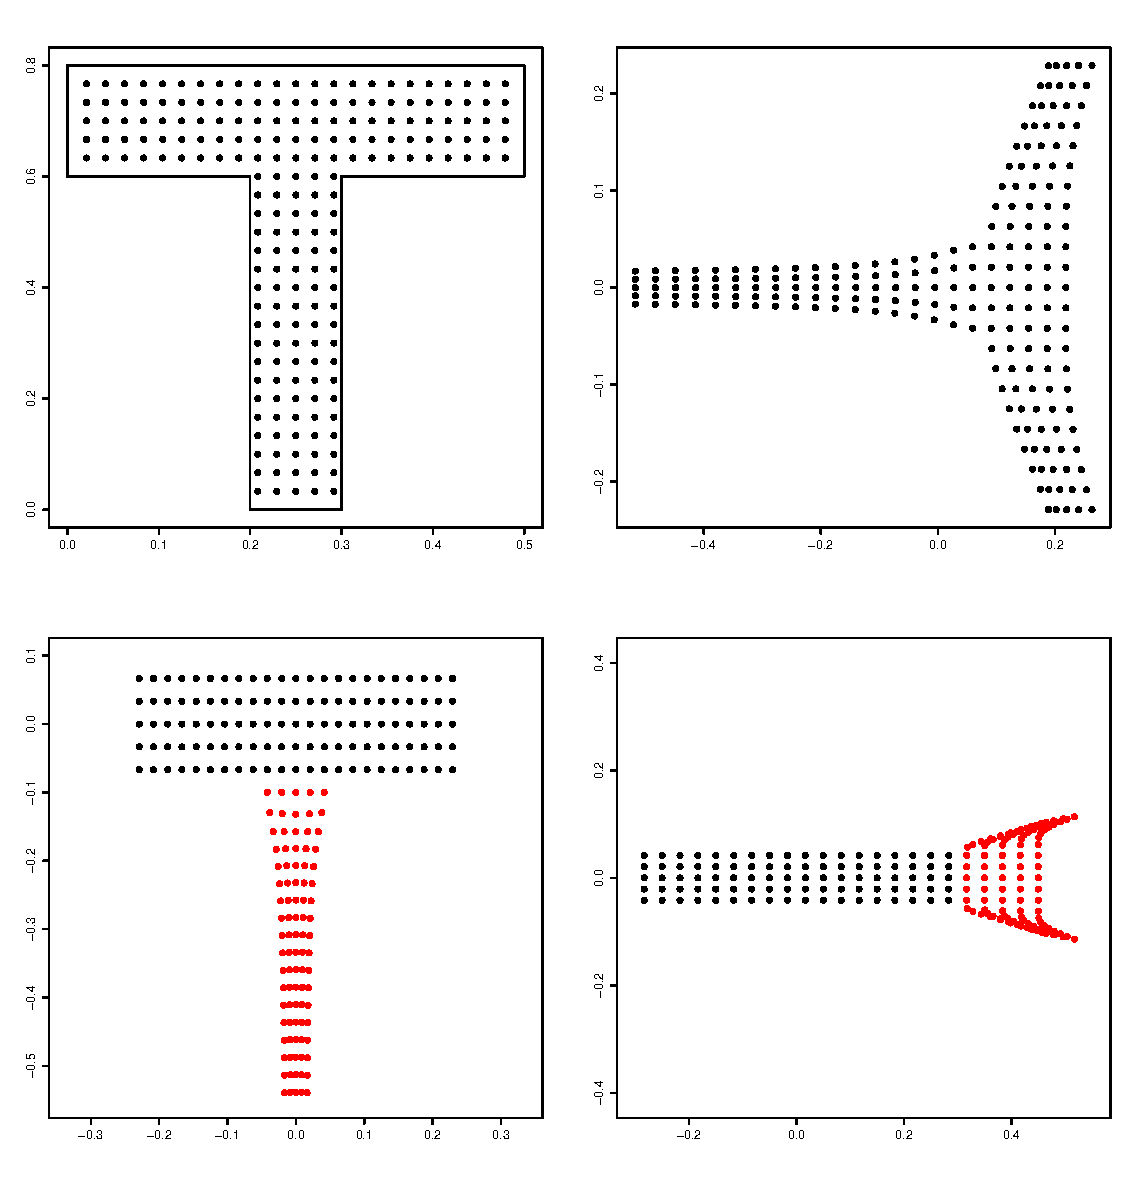
\includegraphics[width=3.5in]{mds/figs/tshape.pdf} \\
\caption{Data generated inside a T-shape (top left) is fed into MDS at once (top right). When either the head or tail of the T is used for the original MDS configuration and the other points inserted, the shape produced is distorted.}
\label{tshape}
% generated using figs/gridtest.R
\end{figure}

Although the cases show in \fig{tshape} are somewhat pathological, looking at more reasonable situations still leads to wildly different results. In \fig{tshaperand} the black and green points make up the original MDS configuration; the five green points are chosen at random. The red points are then inserted. As can be seen in these four typical realisations, the shape of the MDS space is dependent on those points used to create the initial MDS configuration.

% showing the the grid is necessary using the T shape (random samples
\begin{figure}
\centering
% trim order l b r t
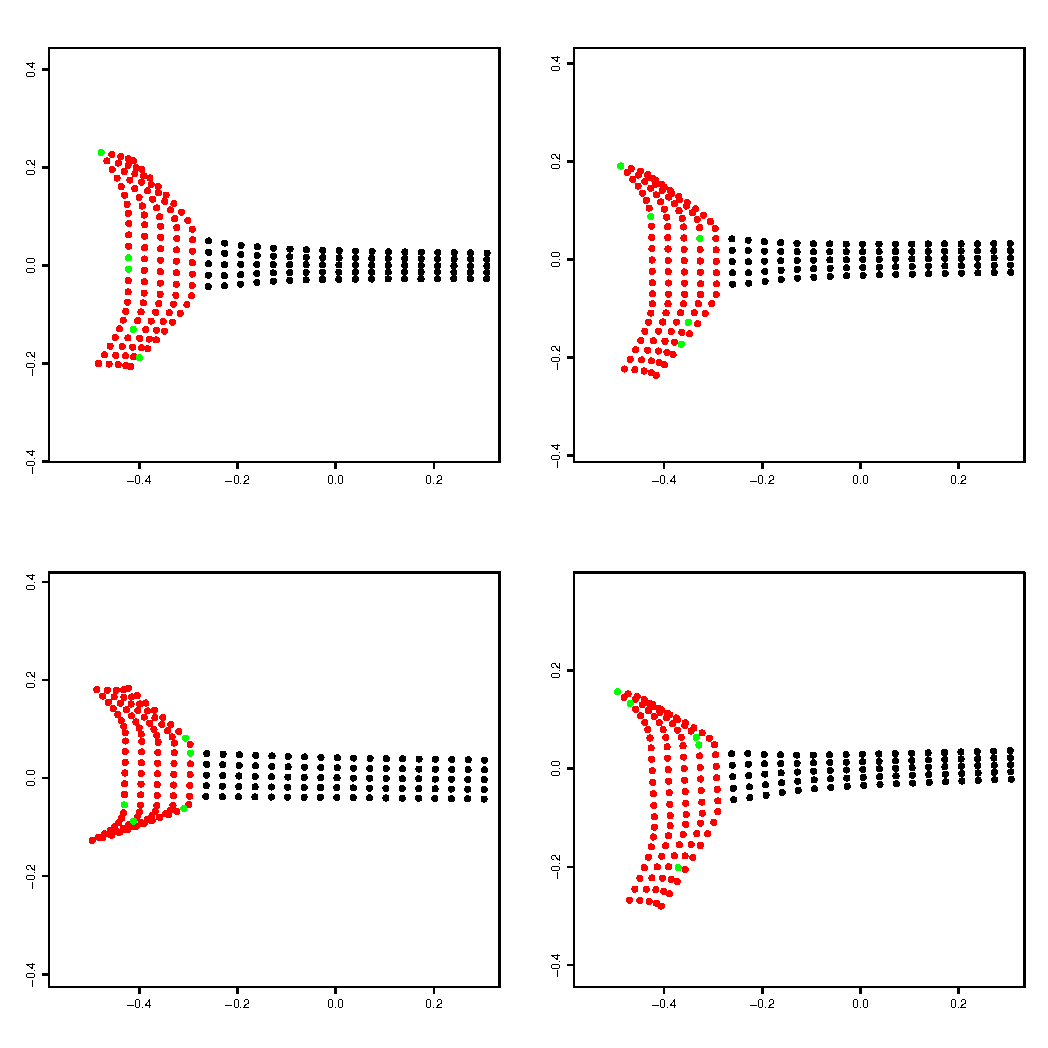
\includegraphics[width=3.5in]{mds/figs/tshaperand.pdf} \\
\caption{Using the T-shape in \fig{tshape} (top left), the tail (black points) of the T was used with 5 randomly sampled (green) points in the head. The head (without the 5 green points) was then inserted into the MDS configuration (red). As can be seen from these four realisations, the output varies greatly depending on the points sampled.}
\label{tshaperand}
% generated using figs/gridtest.R
\end{figure}

Hence, although there are the usual problems with predicting outside of the data, the added problem of the instability of MDS insertion can only confound results further. (Again, this is mentioned at the end of Gower's paper.)

This problem can be rectified by using an appropriately spaced grid on the domain to calculate the eigen-decomposition, thus ensuring that the whole domain is covered. The base MDS configuration is then stable, provided that the grid is fine enough to catch all the features in the boundary of the domain.

\subsubsection{Smoothness of mapping}

Following from this, it is important to make sure that the MDS space is smooth in the sense that a grid of smooth lines over the domain are mapped to a series of smooth lines without discontinuities or sudden changes in direction. Taking the evenly spaced 50 by 50 point grid in \fig{wt2-grid-orig}, first MDS is performed on a dense point set of size 1253, and then a less dense grid is inserted using the method of Gower. The grid produced under the insertion can be seen in \fig{wt2-grid-full}. Taking a sample of 250 points from the 1253, an MDS configuration was also found and the same grid inserted (see \fig{wt2-grid-samp}). From this it is clear that those points mapped into the domain are smooth but in the sample case the features in the far right of the shape (the less pronounced peninsulae) are slightly squashed.

% grid to map
\begin{figure}
\centering
% trim order l b r t
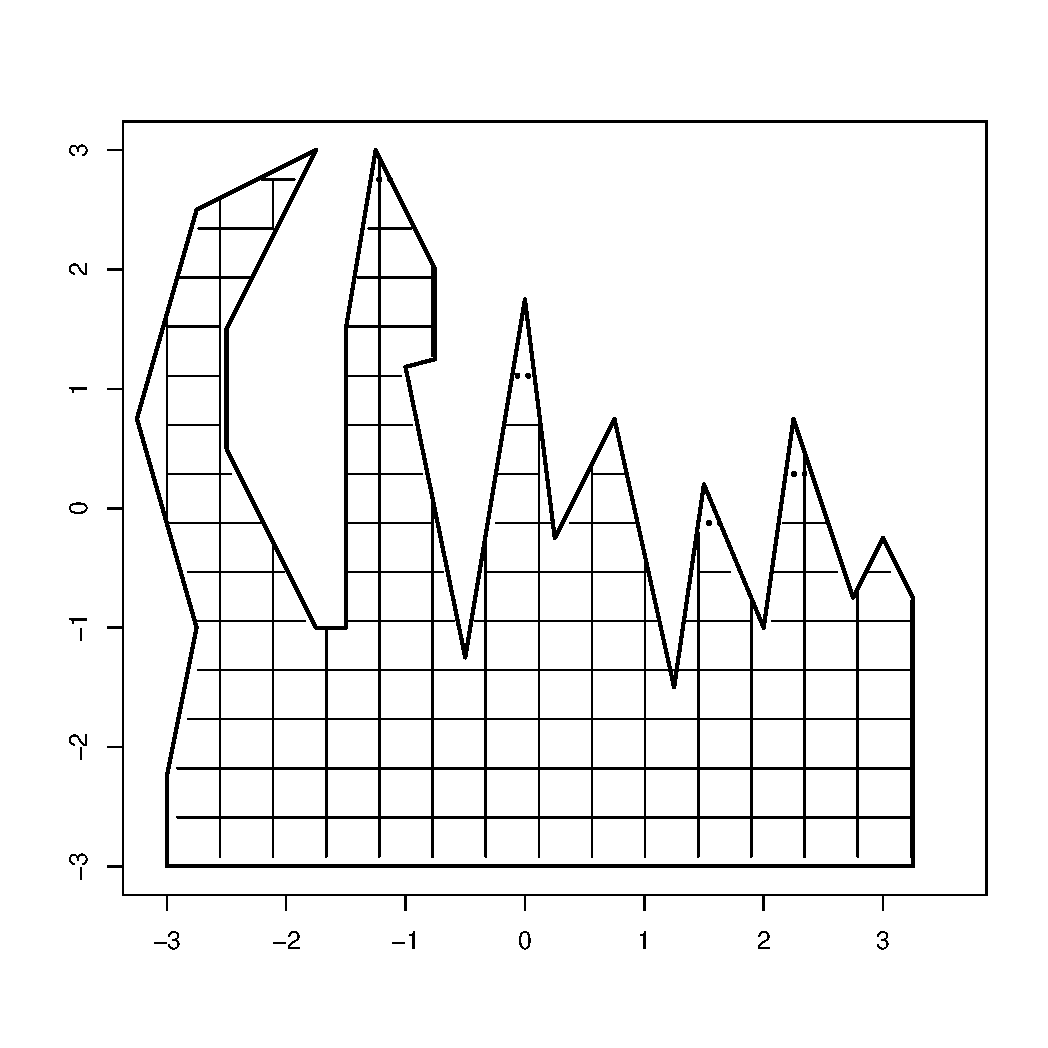
\includegraphics[width=4in]{mds/figs/wt2-grid-orig.pdf} \\
\caption{The grid to be inserted into the MDS configuration over the peninsula domain to test the smoothness of the mapping.}
\label{wt2-grid-orig}
% generated using wt2-grid.R
\end{figure}

% mapped grid (full)
\begin{figure}
\centering
% trim order l b r t
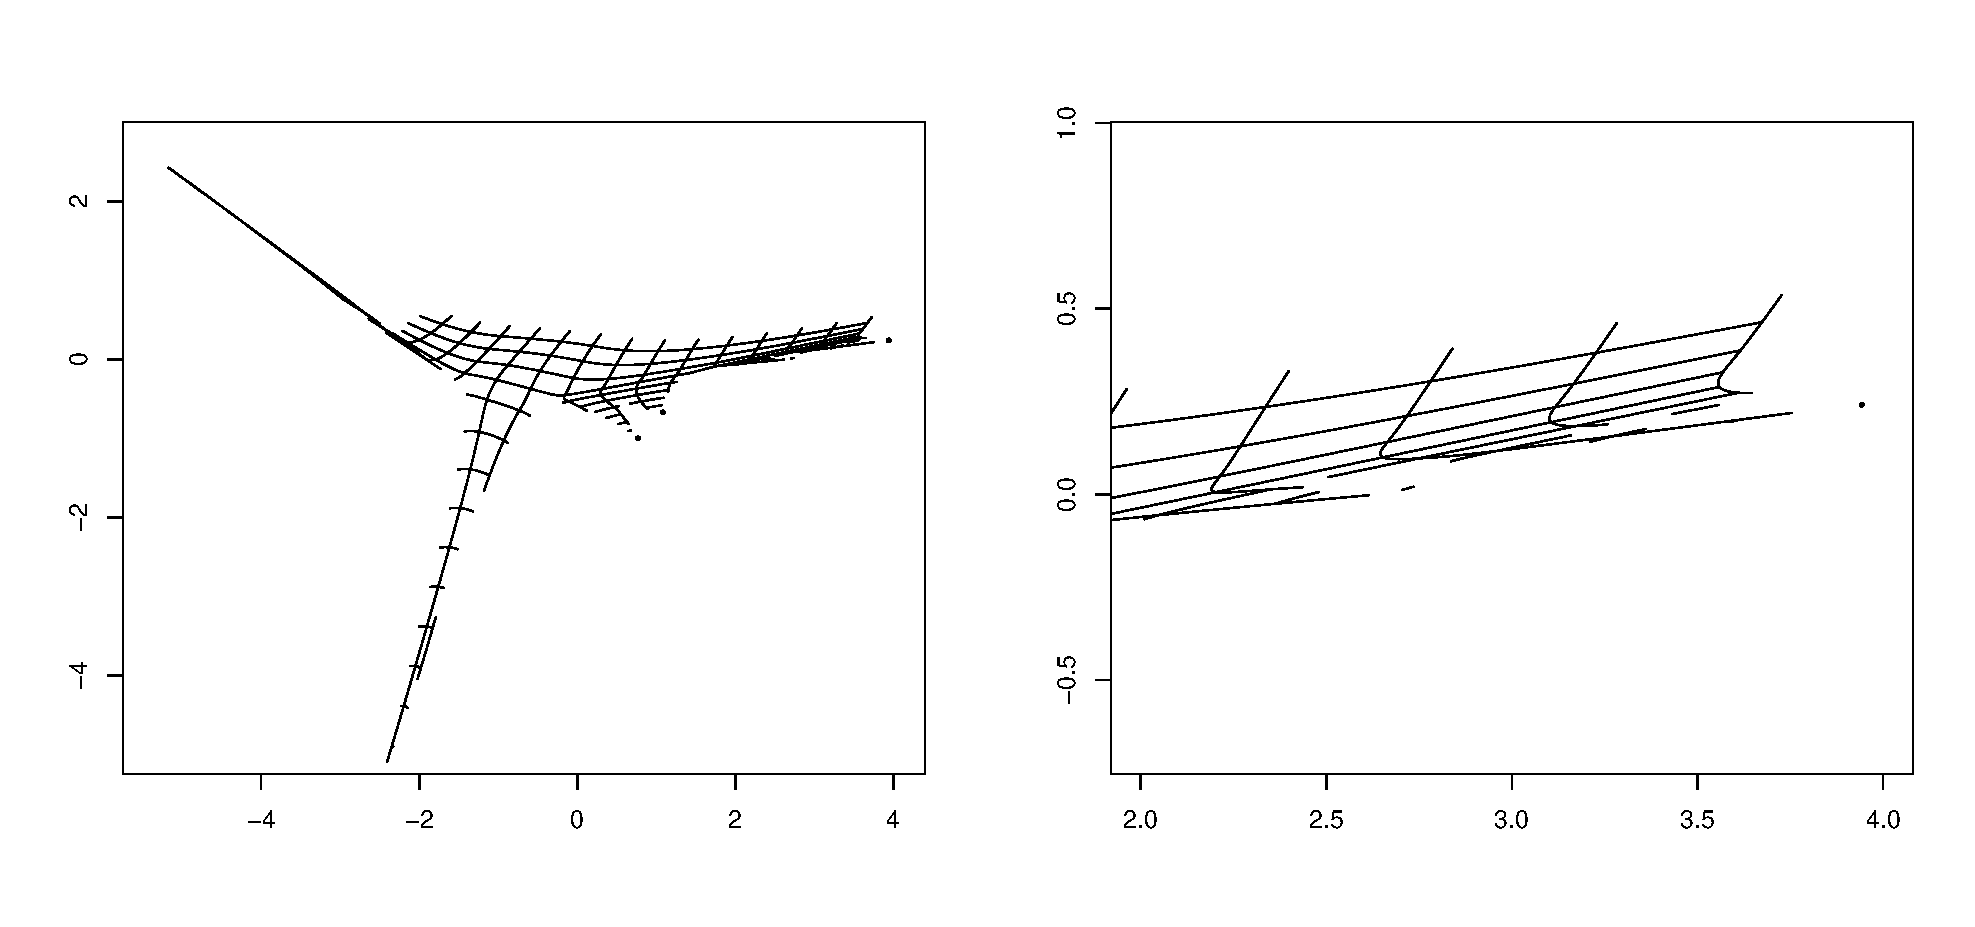
\includegraphics[width=5in]{mds/figs/wt2-grid-full.pdf} \\
\caption{Inserted grid when 1253 points are used to create the initial MDS configuration. The right panel shows a zoom of the far right part of the configuration.}
\label{wt2-grid-full}
% generated using wt2-grid.R
\end{figure}

% mapped grid (samp)
\begin{figure}
\centering
% trim order l b r t
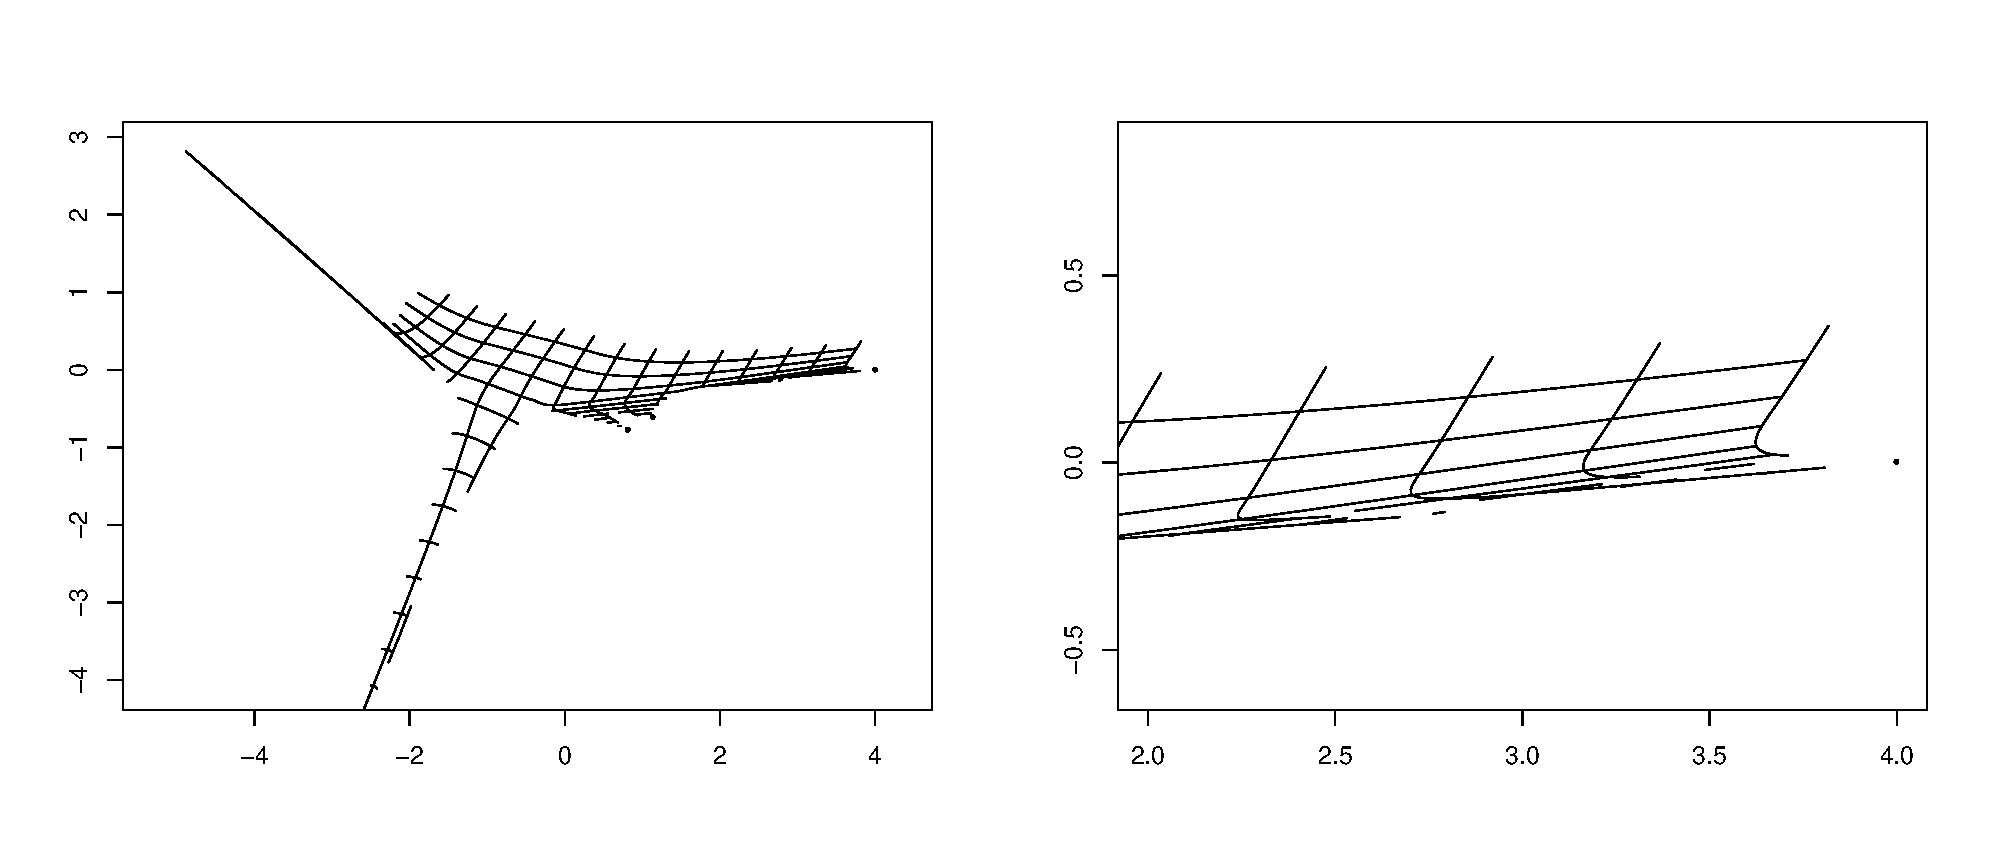
\includegraphics[width=5in]{mds/figs/wt2-grid-samp.pdf} \\
\caption{Inserted grid when 250 randomly chosen points are used to create the initial MDS configuration. The right panel shows a zoom of the far right part of the configuration. Comparing this to that of \fig{wt2-grid-full}, one can see that the features on the right have been squashed together.}
\label{wt2-grid-samp}
% generated using wt2-grid.R
\end{figure}

In conclusion, the mapping can be both reliable and also produces a smooth configuration of points provided that the initial MDS configuration covers the space in sufficient detail.


\section{Finding the within-area distances}
\label{mdsdist}
In order to perform multidimensional scaling the matrix of distances must be found. This section describes a novel algorithm to find the within-area distances.

Let the domain boundary be some polygon, $\Gamma$. Given that there is no direct path within the domain between two points ($p_1$ and $p_2$, say), the algorithm proceeds as follows to create a path (ie. an ordered set of edges and vertices), $\mathcal{P}$:

\begin{enumerate}
\item (INIT) Start by drawing a line between $p_1$ and $p_2$ (\fig{wdia}, ($i$)). Start the path as the lines from $p_1$, $p_2$ to their nearest intersection with the boundary of $\Gamma$ ($p_1^1$, $p_2^1$, say.) Then form two paths. The first path from $p_1^1$ to $p_2^1$ ($\mathcal{P}_1$) contains the vertices of $\Gamma$ found moving along the boundary from $p_1^1$ to $p_2^1$. The second ($\mathcal{P}_2$), is found by taking those vertices on the boundary from $p_2^1$ to $p_1^1$, ie. the vertices of $\Gamma$ not in the first path. It is easy to see that $\{\mathcal{P}_1 \cup \mathcal{P}_2\} \setminus \{p_1^1, p_2^1\} = \Gamma$. The DELETE step (below) is then performed on $\mathcal{P}_1$ and $\mathcal{P}_2$, removing any superfluous vertices. Finding the length of $\mathcal{P}_1$ and $\mathcal{P}_2$ and choosing the shorter ($\mathcal{P^*}$), the initial path is formed as $\mathcal{P}=(p_1,p_1^1,\mathcal{P}^*,p_2^1,p_2)$. 

In \fig{wdia}, ($iii$), $\mathcal{P}_1$ is marked in green and is chosen to form the initial path, $\mathcal{P}=(p_1,p_1^1,\mathcal{P}_1,p_2^1,p_2)$, as $\mathcal{P}_1$ is shorter than $\mathcal{P}_2$, in red.

\item (DELETE) Given a triple of vertices, $(v_i, v_{i+1}, v_{i+2}) \in \mathcal{P}$ , if the line between $v_i$ and $v_{i+2}$ is shorter than the path $(v_i, v_{i+1}, v_{i+2})$ and the line between $v_i$ and $v_{i+2}$ lies inside $\Gamma$ then delete $v_{i+1}$ (\fig{wdia}, ($iv$) and ($vi$).) The entire path is iterated over deleting all superfluous vertices until there are no changes in successive runs. 

For example in \fig{wdia} ($iii$), $v_2$ is deleted from $\mathcal{P}$ because the path straight between $v_1$ and $v_3$ is shorter, and within $\Gamma$.

\item (ALTER) Given a triple of vertices $(v_i, v_{i+1}, v_{i+2})$, if the path $\mathcal{P}_{ID}$ is shorter than the path $(v_i, v_{i+1}, v_{i+2})$ then replace $(v_i, v_{i+1}, v_{i+2})$ with $\mathcal{P}_{ID}$ (\fig{wdia}, ($v$)). The candidate replacement path, $\mathcal{P}_{ID}$, is calculated by running INIT with $p_1$ and $p_2$ replaced by $v_i$ and $v_{i+2}$, producing $\mathcal{P}_I$, and then using DELETE on $\mathcal{P}_I$ to remove superfluous vertices, giving $\mathcal{P}_{ID}$.

For example in \fig{wdia} ($iv$), the path $(v_1, v_2, v_3)$ is longer than the path $\mathcal{P}_{ID}=(v_1, v^1_2, v_3)$ (green dashed line in ($iv$)) so the former is replaced with the latter in $\mathcal{P}$. The path created by INIT is marked as $\mathcal{P}_{I}$ in  ($iv$) in red.

\item (ITER) We then iterate between the DELETE and ALTER steps until there has been no change from one run to the next (ie. convergence) or there have been too many iterations (\fig{wdia}, ($vi$).)
\end{enumerate}

% diagram for finding the shortest path in W
\begin{sidewaysfigure}
\centering
% trim order l b r t
\psfrag{exp1}[]{$\mathcal{P}_1$}
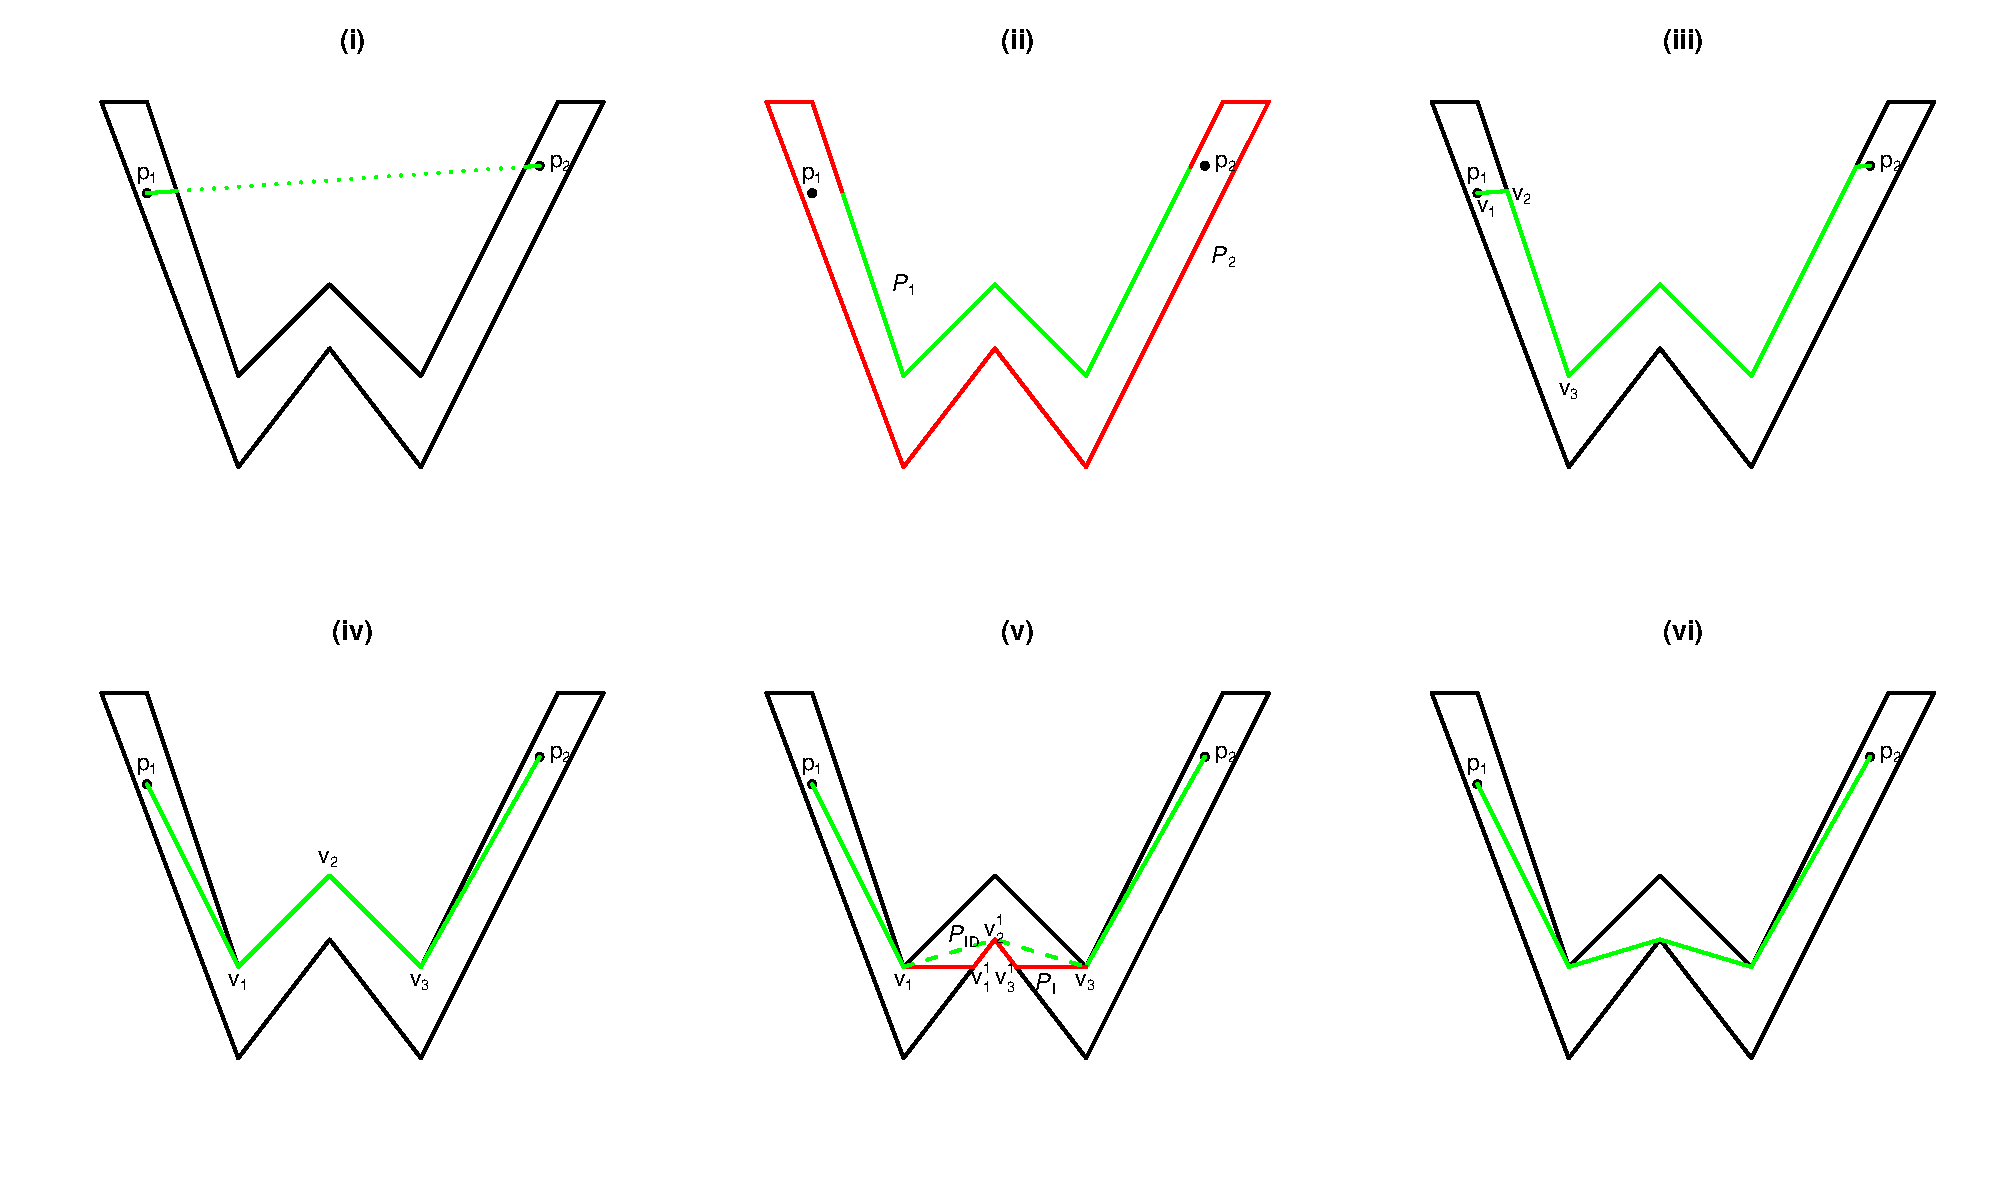
\includegraphics[trim=0in 0.5in 0in 0.25in, width=9.5in]{mds/figs/wdia.pdf} \\
\caption{The green lines in ($i$) to ($vi$) show the steps forming the shortest path as the algorithm progresses from initial state to final, shortest path (bottom right). See \secref{mdsdist}.}
\label{wdia}
% generate /phd-smoothing/mds-writeup/figs/distanceexplanation.R
\end{sidewaysfigure}

Of course, if there is a direct path between $p_1$ and $p_2$ then the Euclidean distance between the points can be used.

\section{Simulation experiments}
\label{mdssims}

Some kind of intro to this stuff here!

In all cases smoothing parameter estimation was performed using GCV.



\subsection{The Ramsay horseshoe}

Again, we start with the modified Ramsay horseshoe since it clearly illustrates the problem of leakage; if a general method is to be useful it must first perform well on even a simple case such as this.

\subsubsection{Setup}

For the horseshoe, samples of 250 points with normal errors (at 3 levels:  $\sigma= 0.1$, 1 and 10) were taken. (These are the settings used in \cite{soap}.) Using these samples, three models were fitted to the data. Predictions were then made over 718 points (including the sample locations). 200 realisations were generated and the EDF and MSE recorded for each replicate. The three models fitted were as follows (using the \textsf{R} packages \texttt{mgcv} and \texttt{soap} with additional bespoke software for finding the within-area distances):

\begin{enumerate}
\item \emph{Thin plate spline}: bivariate \tprs with basis size 100.
\item \emph{Soap film smoother}: 32 knots evenly spread over a grid over the domain, cyclic spline on the boundary was of basis size 39.
\item \emph{MDS}: Used a thin plate spline of basis dimension 100. The initial MDS grid was 20 points wide by 10 points tall.
\end{enumerate} 

Note that due to time and computational restrictions, the boundary was reduced from the 160 vertex polygon in the \texttt{fs.boundary()} function in \texttt{soap} to a 21 vertex polygon by only using every 8$^\text{th}$ vertex. This should not cause a major difference in results even if the soap film used the full boundary and the MDS used only the reduced set of edges, since objective is to allow the smoother to get a broad idea of the topology of the domain, rather than the minutiae of the boundary features.

\subsubsection{Results}

Predictions from a typical realisation can be seen from \fig{mds-ramsay-fit-1}, where $\sigma=1$ with a sample size of 250. Both the soap film smoother and MDS are able to reproduce the main features of the true horseshoe function due to their ability to respect the boundary (in the case of the soap film) or the geometry of the domain (in the case of MDS.) The \tprs shows leakage as expected. This is reflected in table \ref{ramsayresultstable} where we see that the soap film smoother and MDS have significantly smaller average MSE. When the noise level is high the MDS approach outperforms the soap film smoother in MSE terms (and is less variable).

\begin{table}[ht]
\centering
\begin{tabular}{c c c c}
 & & MSE & \\ 
$\sigma$ & MDS & Soap film & Thin plate\\ 
\hline
0.1  & 0.0032 (3$\cross10^{-5}$) & 0.0022 (3$\cross10^{-5}$) & 0.0402 (0.0008) \\ 
1  & 0.0436 (0.0015) & 0.0482 (0.0014) & 0.2306 (0.0024) \\ 
10  & 2.0652 (0.1215) & 3.0702 (0.2382) & 3.3713 (0.1133) \\ 
\end{tabular}
\begin{tabular}{c  c c c }
&  & EDF & \\ 
$\sigma$ & MDS & Soap film & Thin plate\\ 
\hline
0.1 & 47.613 (0.3497) & 39.164 (0.26) & 92.5996 (0.1020)\\ 
1  & 8.3828 (0.3452) & 11.868 (0.4010) & 46.607 (0.4238)\\ 
10 & 5.0577 (0.3324) & 5.5863 (0.2876) & 5.9786 (0.2511)\\ 
\end{tabular}
\caption{Mean MSE and estimated degrees of freedom (EDF) for the three models fitted to the modified Ramsay horseshoe function with standard errors (in brackets) over 200 realisations. Sample size was 250 with error levels given in the column marked $\sigma$.}
\label{ramsayresultstable}
\end{table}

The EDFs in table \ref{ramsayresultstable} show that the MDS approach fits a less complex model than the thin plate spline on average, and for the two higher error situations, has a lower EDF than the soap film. Given that this is coupled with a lower MSE, it appears that the MDS approach simultaneously yields both a more accurate and less complex model than the soap film for the horseshoe when there is a high level of noise. When noise is lower, the soap film and MDS MSEs are still of the same order.

% Ramsay fit with error=1 
\begin{figure}
\centering
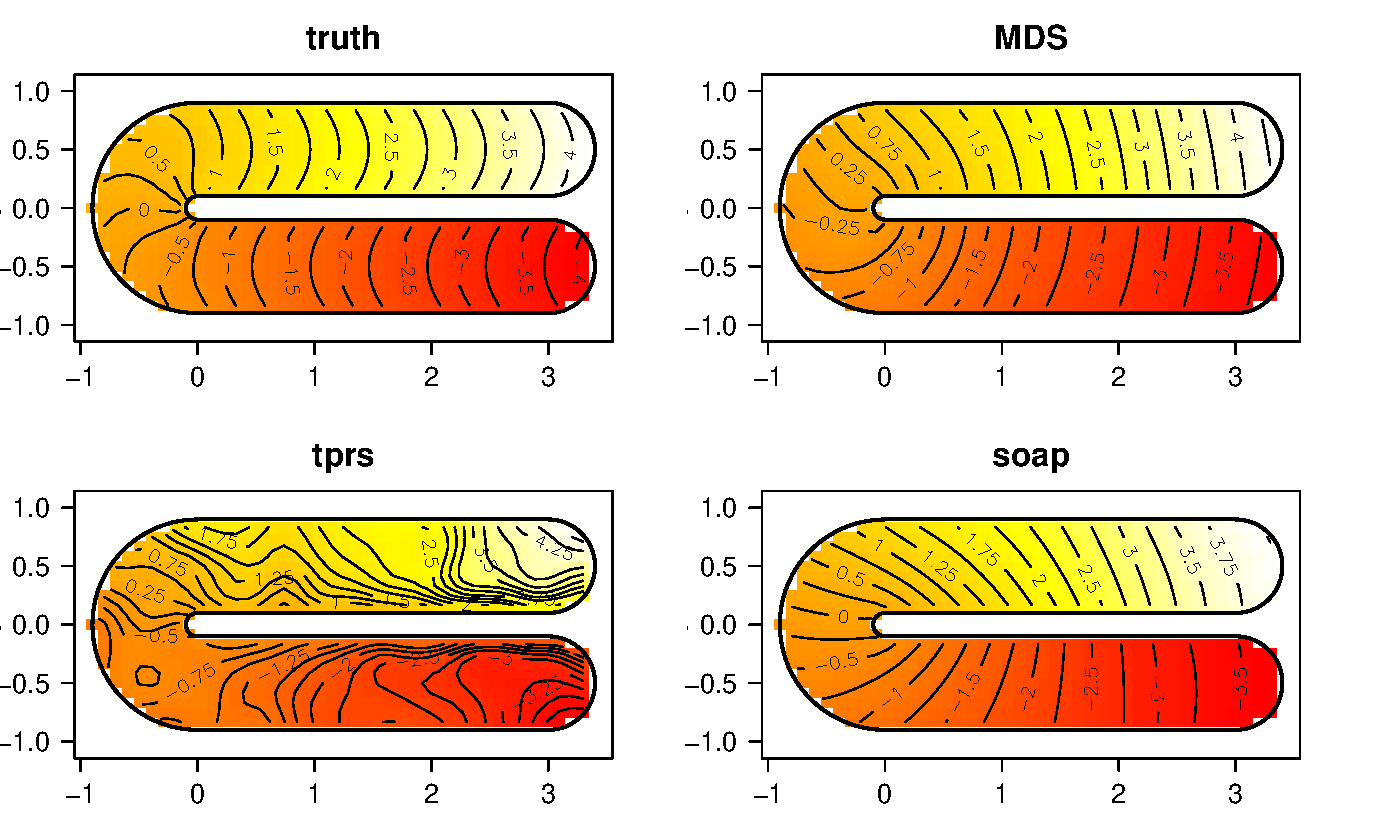
\includegraphics[width=6in]{mds/figs/ramsay-fit-1.pdf} \\
\caption{Top left: truth for the (modified) Ramsay horseshoe. Others: a typical realisation of fits from the three models when 250 points are sampled with noise set to $\sigma=1$.}
\label{mds-ramsay-fit-1}
% generated (roughly) using ramsay-smooth-test.R
\end{figure}

Just as when the \sch transform was used to morph the domain, it is interesting to see what has happened to the distribution of points in space. \Fig{mdsrampoints} shows the effect of the transform on a regular grid of points (left) when they are projected into MDS space (right.) The projection has also succeeded in parting the two arms of the horseshoe, reducing leakage (as can be seen in the realisations in \fig{mds-ramsay-fit-1}).

\begin{figure}
\centering
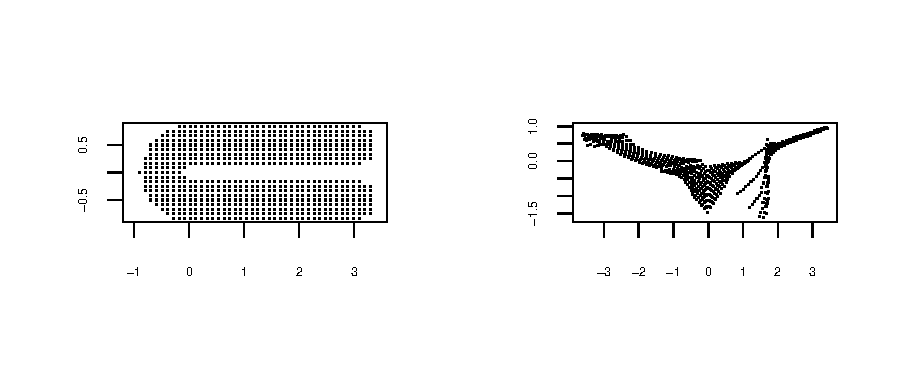
\includegraphics[width=6in,trim=0.5in 0.5in 0in 0.5in]{mds/figs/mdsrampoints.pdf} \\
\caption{A regular grid over the Ramsay horseshoe (left) and its projection into MDS space (right).}
\label{mdsrampoints}
% generated using thesis/mds/figs/mdsrampoints
\end{figure}


\subsection{Peninsulae domain}

The Ramsay horseshoe is an easy domain to smooth over since it is obvious how the transformation should be distorting space. For this reason a more realistic, complex domain would provide a better insight into the efficacy of the method. The domain shown in \fig{wt2-truth} is an approximation to a coastline with a strong trend along both peninsulae (in a manner similar to that of the horseshoe) but with the added complication of a further peak in the lower right corner.

\subsubsection{Setup}

The simulations consisted of 200 realisations of 250 samples from the surface in \fig{wt2-truth}. Normal errors were added at three levels $\sigma=0.35$, 0.9 and 1.55 (corresponding to signal-to-noise ratios (SNRs) of 0.95, 0.75 and 0.5, respectively. SNRs were calculated as the mean squared correlation between true function value and the truth with error added.) Mean squared error over 1253 prediction points (including those points in the sample) was calculated and recorded, along with EDF for each model. The models fitted were:

\begin{enumerate}
\item \emph{Thin plate spline}: bivariate thin plate spline with basis size 100. 
\item \emph{Soap film smoother}: cyclic spline on boundary of basis size 60, 109 internal knots evenly spaced over the domain on a grid.
\item \emph{MDS}: after transform a bivariate thin plate spline with basis size 100 was fit. The initial MDS grid was 74 points square.
%\item \emph{MDS with tensor product}: tensor product of two thin plate splines, each of basis dimension 12. The initial MDS grid was 74 points square.
\end{enumerate} 

\subsubsection{Results}

Looking at a typical realisation in \fig{wt2-fit-0.5}, we see that soap (bottom right panel) does very well, as can be expected, and the thin plate spline (\fig{wt2-fit-0.5}, bottom left panel) fit shows leakage (again, as can be expected.) 

% wt2 truth 
\begin{figure}
\centering
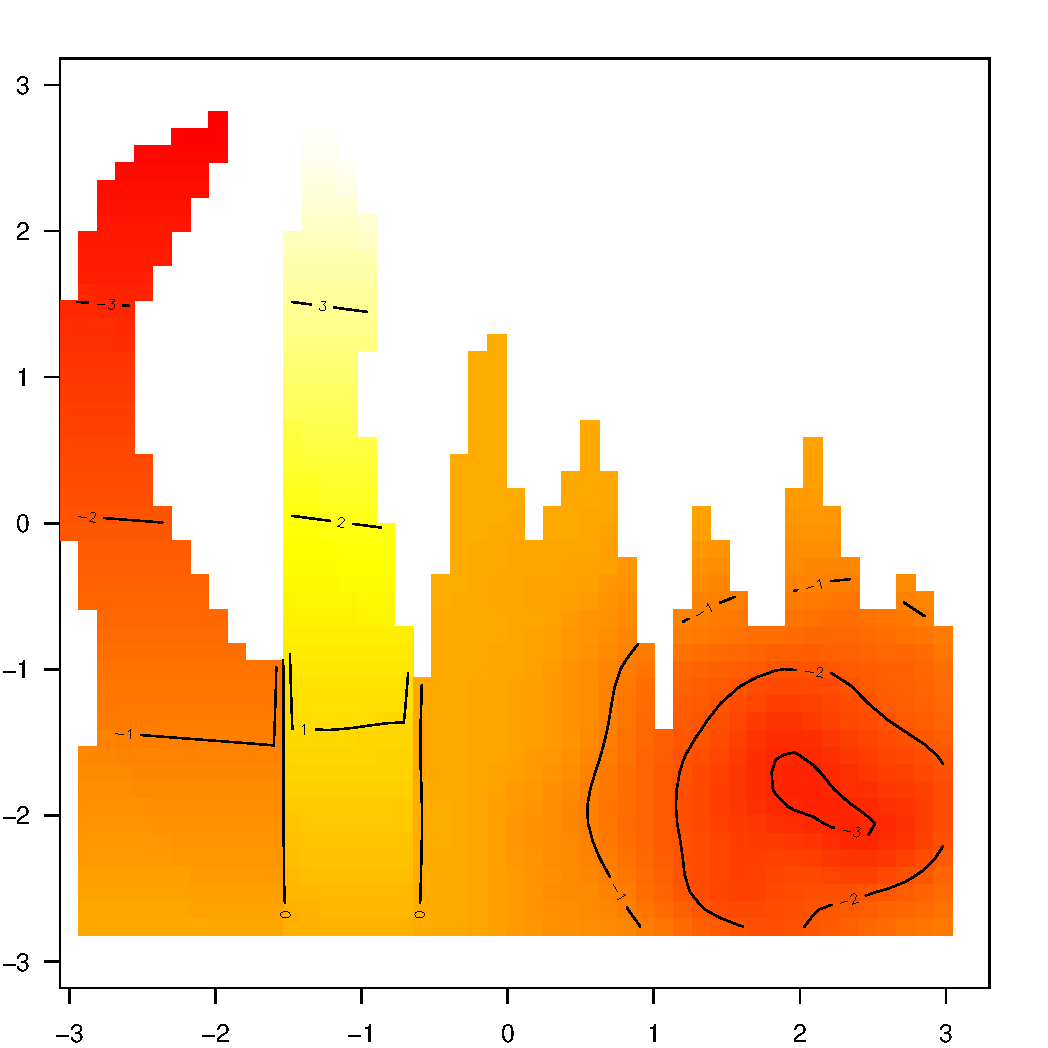
\includegraphics[width=3in]{mds/figs/wt2-truth.pdf} \\
\caption{True function for the domain with multiple peninsulae.}
\label{wt2-truth}
% generated (roughly) using wt2-smooth-test.R
\end{figure}

%The final model, above, was chosen after it appeared that the MDS with a bivariate thin plate spline did not adequately model the peak in the right corner of the domain (\fig{wt2-fit-0.5}, top left panel.) After using a tensor product of thin plate splines a better fit to the right peak was found (\fig{wt2-fit-0.5}, top right panel), although this is not reflected particularly well in terms of mean squared error (see table \ref{wt2resultstable}.) The visual improvement in fit can be explained by thin plate splines in two dimensions being an isotropic smooth and since space has not been transformed in a uniform way in both dimensions.

%Table \ref{wt2resultstable} shows that when there is low error, both the soap film and thin plate splines outperform the MDS approach, but once the errors are increased the MDS does much better. The MDS approach also benefits from having a smaller EDF than all the other approaches in all of the noise scenarios, the tensor MDS doing better at lower noise levels. This is encouraging and shows that perhaps there is a place for this technique alongside the soap film smoother if the method can be improved for low noise situations.

INVESTIGATE THE ABOVE!!!!

\begin{table}[ht]
\centering
\begin{tabular}{c c c c c}
 &  & MSE  & &\\ 
%$\sigma$ & MDS & MDS (tensor) & Soap film & Thin plate\\ 
$\sigma$ & MDS & Soap film & Thin plate\\ 
\hline
0.35  & 0.07 (0.00062) & 0.0539 (5e-04) &0.082 (0.00104)\\
0.9  & 0.177 (0.00184) & 0.1308 (0.00197) &0.1938 (0.00241)\\
1.55  & 0.2859 (0.00438) & 0.2362 (0.00434) &0.3509 (0.00471)\\
%0.05  & 0.0948 (0.00084) & 0.0603 (0.00352) & 0.0237 (0.00039) &0.0504 (0.00039) \\ 
%0.5  & 0.1426 (0.00078) & 0.1106 (0.00133) & 0.1013 (0.02151) &0.1123 (0.02151) \\ 
%5  & 0.9179 (0.02644) & 1.2481 (0.04159) & 1.1987 (0.04111) &1.3865 (0.04111)\\ 
\end{tabular}
\begin{tabular}{c c c c c}
 &  & EDF  & &\\ 
%$\sigma$ & MDS & MDS (tensor) & Soap film & Thin plate\\ 
$\sigma$ & MDS & Soap film & Thin plate\\ 
\hline
0.35 &80.9039 (0.57103) & 55.6979 (0.51448) & 77.9619 (0.46726)\\ 
0.9 &35.0185 (0.76449) & 29.7171 (0.57477) & 48.0508 (0.47636)\\ 
1.55 &19.4625 (0.57265) & 20.2918 (0.36634) & 32.2715 (0.47961)\\ 
%0.05 &72.262 (0.89606) & 78.2691 (0.679) & 94.5187 (0.78697) & 86.9415 (0.78697)\\ 
%0.5 &40.7981 (0.46687) & 50.5025 (0.36223) & 45.2341 (0.74063) & 58.418 (0.74063)\\ 
%5  &6.8274 (0.36097) & 8.577 (0.3649) & 11.5419 (0.83982) & 11.9407 (0.83982)\\ 
\end{tabular}

\caption{Mean MSE and EDF for the four models fitted to the peninsula domain with standard errors (in brackets) over 200 realisations.}
\label{wt2resultstable}
\end{table}

% wt2 fit with error=0.5
\begin{figure}
\centering
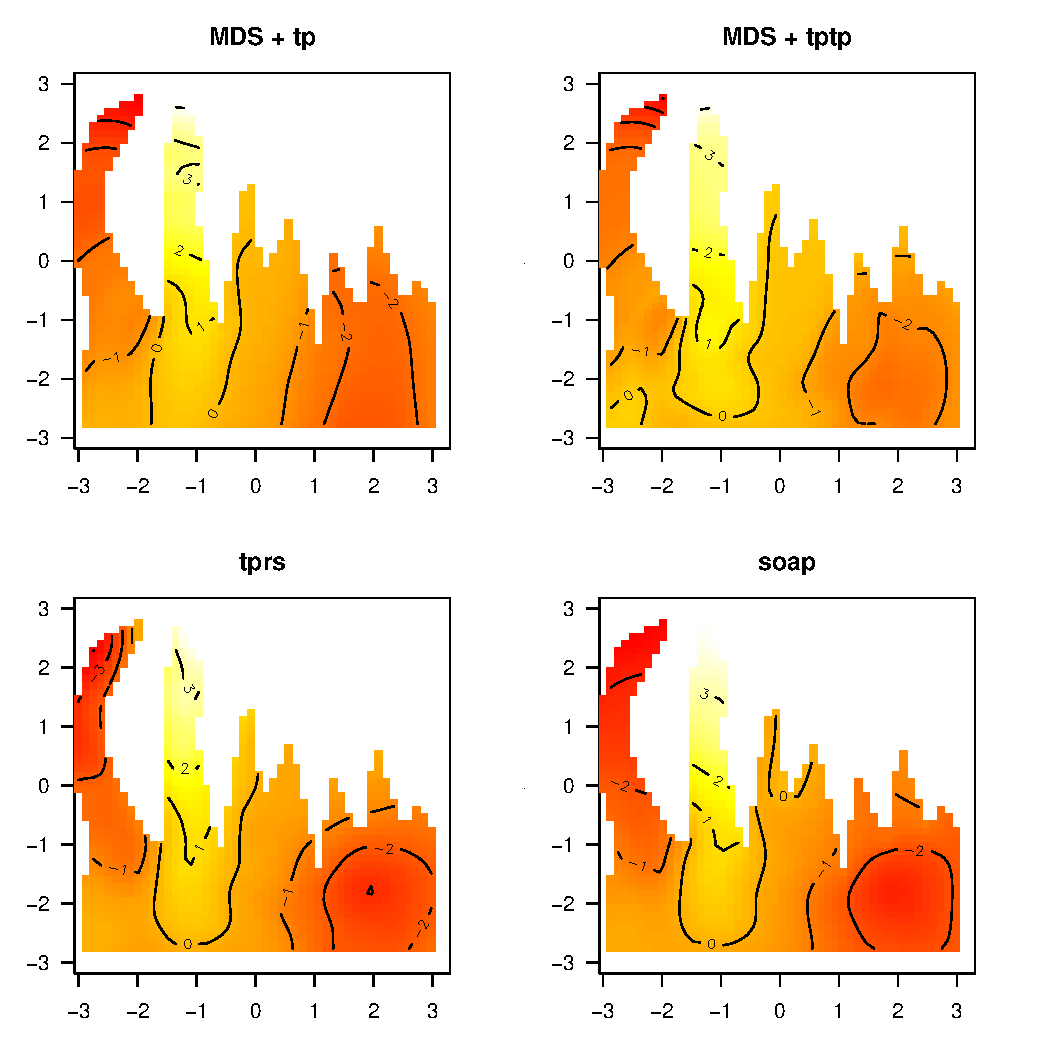
\includegraphics[width=6in]{mds/figs/wt2-fit-05.pdf} \\
\caption{A typical realisation of fits from the multiple peninsulae domain when $\sigma$ is set to 0.5.}
\label{wt2-fit-0.5}
% generated (roughly) using wt2-smooth-test.R
\end{figure}

As with the Ramsay horseshoe, it is interesting to see what the projection into MDS space has done to the distribution of the points in the domain. \Fig{mdswt2points} shows

% how the points are projected for wt2
\begin{figure}
\centering
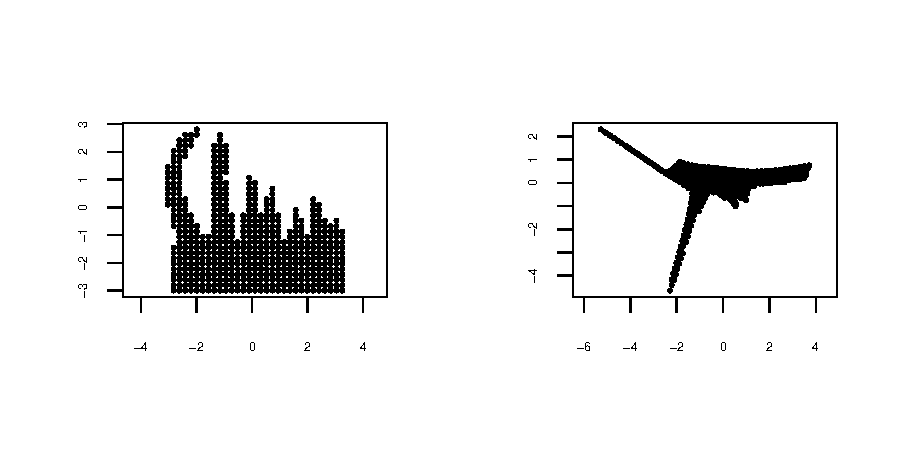
\includegraphics[width=6in,trim=0.5in 0.5in 0in 0.5in]{mds/figs/mdswt2points.pdf} \\
\caption{A regular grid over the peninulae domain (left) and its projection into MDS space (right.)}
\label{mdswt2points}
% generated using thesis/mds/figs/mdswt2points
\end{figure}

\section{Improvements}
\label{MDSimprov}
